\section{Snake game}
\label{sec:snake}

In this section the implementation of the Snake game is presented. Here only the parameters of the game itself and an example of the screen are shown. The documentation of the source code is automatically generated using Doxygen \cite{DOXYGEN} with Travis~CI \cite{TRAVIS} and available in Reference~\cite{MyDOXYGEN}.\\

The code has been developed in Java language, based on the tutorial in Reference~\cite{JAVA}. The game is played through the arrow keys with a frequency of $150$~$\mu$s. The snake moves at this frequency and only one command for each time unit is allowed. The snake is enlonged for each eaten apple and the game ends when the snake hits the borders or itself.\\

The parameters for the playground size, initial position and dimensions of snake and apples, and snake speed are given in Table~\ref{tab:snake_parameters}. The result of the game is shown in Figure~\ref{fig:game_screen}. This game is used to train the Neural Network.


\begin{table}[b]
\centering
\begin{tabular}{@{}lll@{}}
\toprule
\multicolumn{3}{@{}l}{Parameters of the Snake game}\\
\midrule
\multicolumn{3}{@{}l}{\emph{Playground}}\\
Dimensions & \phantom{aaa} &  $(400\times400)$~pt\\
Segmentation matrix & \phantom{aaa} &  $(20\times20)$\\[2mm]

\multicolumn{3}{@{}l}{\emph{Initial coditions}}\\
Apple position & \phantom{aaa} &  $(200,200)$~pt\\
Apple dimension & \phantom{aaa} & 1~grid segmentation\\
Snake head position & \phantom{aaa} &  $(300,200)$\\[2mm]
Number of snake blocks & \phantom{aaa} &  2 (vertically-disposed)\\[2mm]

\multicolumn{3}{@{}l}{\emph{Game speed}}\\
Clock period & \phantom{aaa} &  $150~\mu$s\\

\bottomrule
\end{tabular}
\caption{Parameters of the Snake game. The numbers are used in input to determine size and initial conditions of the game \cite{MyDOXYGEN}.}
\label{tab:snake_parameters}
\end{table}

\begin{figure}[b]\centering
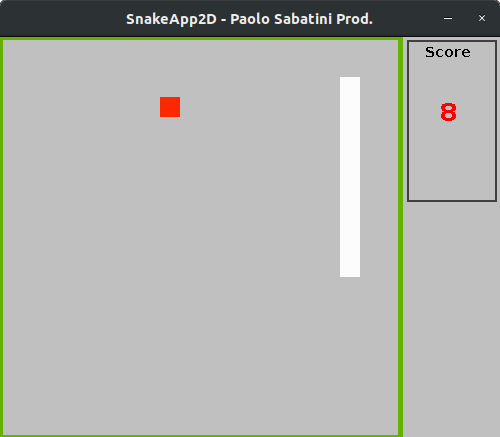
\includegraphics[width=0.42\textwidth]{imgs/SnakeScreen.png}
\caption{Screen of the game.}
\label{fig:game_screen}

\end{figure}